\chapter{Prosessdokumentasjon}
\lettrine[lines=2]{I}{} følgende kappitel beskriver vi hvordan hele utviklinsprosessen for protitypene har foregått. Hensikten er at man skal illustrere hele prosessen fra idé, mockup til hi-hi prototype klar for brukertesting. 

\section{Første utkast}


\begin{figure}[ht]
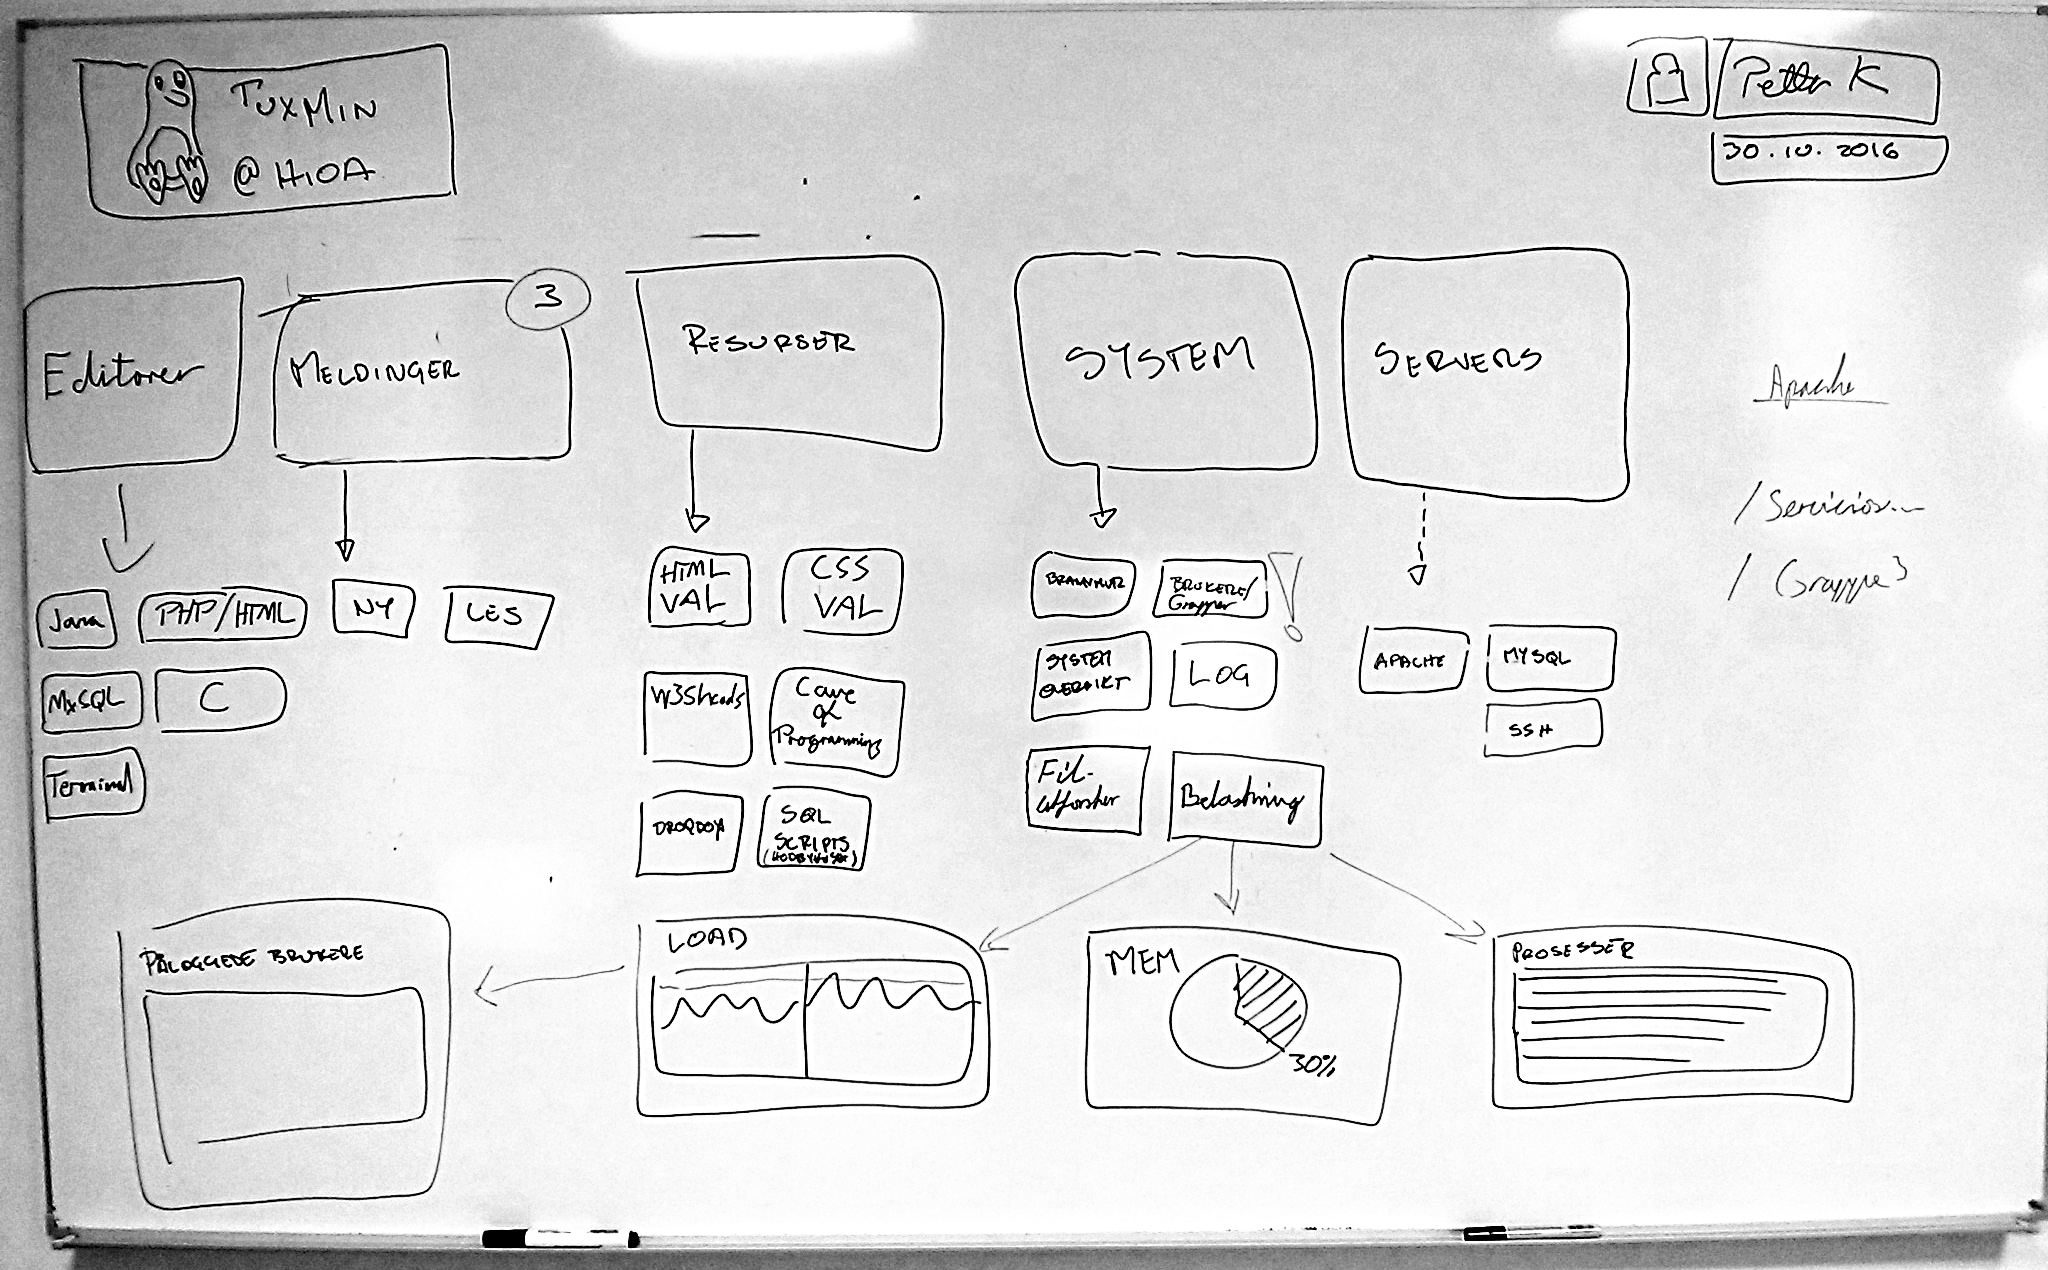
\includegraphics[width=\textwidth,height=\textheight,keepaspectratio]{./img/prosessdokumentasjon/foersteutkast/foerste.jpg}
\caption[Første utkast]{Første utkast over brukergrensesnittet.}
\label{fig:foersteutkast}
\end{figure}

\section{Low-fi prototype}

\section{Hi-fi prototype}

\section{Kriterier og avgjøresler}
Fokuser på alle valg som ble tatt. Hvilke kriterier og 
prinsipper i faget ligger bak avgjørelsene? 

Her kan vi skrive om hvorfor vi har akkuratt valgt Linux. Hvorfor skal løsningen være webbasert og hvorfor skal den kjøres i en virtuell maskin? Og så andre kriterier og avgjøresel som vi har tatt under veien. 